\documentclass{article}

\usepackage{amsmath,amsfonts,amssymb}
\usepackage[landscape]{geometry}
\usepackage{graphicx}
\usepackage{ pstricks,pst-grad  }
\usepackage{wrapfig}
\usepackage{algorithm}
\usepackage[noend]{algpseudocode}
 
\usepackage{color}
\usepackage{epstopdf}
\usepackage{framed}
 

 %  TikZ & PGF Libraries
\usepackage{tikz}
\usepackage{animate}
\usetikzlibrary{arrows}
\usetikzlibrary{positioning}
\usetikzlibrary{decorations.pathreplacing}
\usetikzlibrary{decorations.pathmorphing,patterns}
\usepackage{calc}


 \def \red{\color{red}}
\def \black{\color{black}}
\def \blue{\color{blue}}
\def \brown{\color{brown4}}
 \def \seag{\color{seagreen}}
\definecolor{gold}{rgb}{207,181,59}
%\newcommand{\green}{\color{thegreen}}
\definecolor{OliveGreen}{rgb}{0,0.6,0}

\def \pu{\color{purple4}}
\def \gry{\color{gray}}

\newcommand { \blueline } { \bcenter\blue\hrule width9.5in height3pt \vskip-25pt\black \ecenter }
\newcommand { \redline } { \red\hrule width9.5in height1pt\black }
\newcommand { \doubleredline } { \red\hrule width9.5in height1pt \vskip4pt \hrule width9.5in height1pt\black }
\newcommand {\redtitle}[1] {\blueline \bcenter{\bf\sffamily\red #1  }\ecenter \blueline  }
\newcommand {\bitem} {\begin{itemize} }
\newcommand {\eitem} {\end{itemize} }
\newcommand {\bdes} {\begin{description} }
\newcommand {\edes} {\end{description} }
\newcommand {\benum} {\begin{enumerate} }
\newcommand {\eenum } {\end{enumerate} }
\newcommand {\bcenter} {\begin{center} }
\newcommand {\ecenter} {\end{center} }
\newcommand {\ssp} {  \;    }
\newcommand{\vten} {\vskip10pt}
\newcommand{\vfive} {\vskip5pt}
 
 %  TIKZ
 \newcommand \btikz {\begin{tikzpicture} }
\newcommand \etikz {\end{tikzpicture} }

 


\renewcommand{\familydefault}{\sfdefault}

\textheight=6.5in
\textwidth=9.55in
\oddsidemargin = 0.0 in
\evensidemargin = 0.0 in
\topmargin = 0.0 in
\headheight = 0.0 in
\headsep = 0.0 in
\parskip = 0.2in
\parindent = 0.0in
\hfuzz=20pt
\overfullrule=0pt
%%%%%%%%%%%%%%%%%%%%%%%%%%%%%%%%%%%%%%%%%%%%%%%%


\begin{document}
\pagestyle{empty}

 \sffamily
 
\bcenter
{\large \bf Homework 3 - Polynomial  \& Piecewise Polynomial Interpolation  } \medskip
\ecenter

\vskip.25in
\hrule\smallskip\hrule
\medskip

\benum
\item {\bf  Polynomial interpolation.}   Consider the 3 points $(x_i,y_i)$, $i=1,2,3$ given by (-2,1),  (0,-2),  and (3,1).  We want to first determine the Lagrange form of the interpolating polynomial and then evaluate the polynomial at a given point to given us an approximation there.  That is, we want to write the polynomial as 
$$ p_2(x) = y_1 L_1(x) + y_2 L_2 (x)+ y_3 L_3(x) $$
where each $L_i(x)$ is a quadratic polynomial satisfying $L_i(x_i) = 1 $ and $L_i(x_j) = 0 $ for $i \ne j$.
\benum
\item  Determine the quadratic polynomials $L_1(x), L_2(x), L_3(x)$ and verify that they satisfy the conditions
$$ L_1(x_1) = 1, \quad L_1(x_2)=L_1(x_3)=0 \qquad  L_2(x_2) = 1,\quad L_2(x_1)=L_2(x_3)=0  \qquad
L_3(x_3) = 1, \quad L_3(x_1)=L_3(x_2)=0$$
Simplify each expression and write as $a x^2 + b  x + c$ for constants $a, b, c$.
\item Write out $p_2(x)$ in terms of these 3 quadratic polynomials. You do not have to simplify it.
\item Evaluate the polynomial at $ \displaystyle x=1$. Show your work.
 

\eenum
 
 
\medskip \hrule \medskip
\item   {\bf Piecewise Linear  Polynomial interpolation}.  Consider the 3 points $(x_i,y_i)$, $i=1,2,3$ given by   (0,-2), (-2,1),  and (3,1). 
We want to determine the piecewise linear interpolating polynomial for these points and evaluate it at a point.  
 \benum
 \item Give the number of linear polynomials needed and the interval where each is defined.
\item Determine the  piecewise linear interpolating polynomial for these points; write each line in the form $y(x)= ax + b$ for constants $a$ and $b$.  Be sure to give the interval where each linear polynomial is defined in your definition.
\item Evaluate your piecewise linear interpolant at $x=1$.  Show your work.
\item Compare your result in (c)  with those from (1c).   Are they the same?  Why or why not?
\eenum

\medskip \hrule \medskip

\item{\bf Linear Regression. }  The line which fits the points
$$ (1,3) \quad (2,-2) \quad (3,-1) \quad (4, -5)
$$
using linear regression is $-2.3x+4.5$.  These points and the line are plotted on the next page.  
\benum

\item On the given plot draw the vertical distances whose sum of the squares of these distances are minimized in the regression process.
\item Compute the actual variance (the sum of the squares of the distance from each point to the line).   {\bf Leave your answer as the sum of the squares of numbers}; you do not need to simplify. You may check your answers using Python but you should do this by hand.
\item Using this linear fit to the data, what is the prediction for $x=2.5$?
  \eenum  \eenum
 \bigskip\hrule\smallskip\hrule
\bigskip
\newpage
\bcenter
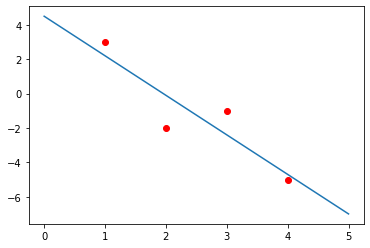
\includegraphics[width=7in] {hwk3}
\ecenter

 
\end{document}

\item   {\bf Piecewise Linear  Polynomial interpolation}.  Consider the 3 points $(x_i,y_i)$, $i=1,2,3$ given by  (0,4), (1,3) and (-1,9). 
We want to determine the piecewise linear interpolating polynomial for these points and evaluate it at a point. (Hint:  Be sure to first order the points from smallest $x$-value to largest.)
 \benum
 \item Give the number of linear polynomials needed and the interval where each is defined.
\item Determine the  piecewise linear interpolating polynomial for these points; write each line in the form $y(x)= ax + b$ for constants $a$ and $b$.  Be sure to give the interval where each linear polynomial is defined in your definition.
\item Evaluate the interpolant at $x=1/2$.  Show your work.
\item Compare your result in (c)  with those from (1c).   Are they the same?  Why or why not?
\eenum
